\documentclass{entcs} 
\usepackage{CSC8498macro}
\usepackage{graphicx}
\graphicspath{{./Images/}}
%% This document describes the formatting instructions for the CSC8498 final report.

\makeatletter

\def\lastname{Boulderstone}
\begin{document}

\begin{frontmatter}
\title{Rollback Netcode, Implmentation and Adoption}
\author{Edward Boulderstone}
  \address{School of Computing Science, Newcastle University, UK} 
\thanks[nigellemail]{Email:
    \href{mailto:E.Boulderstone@ncl..ac.uk} {\texttt{\normalshape
        E.Boulderstone@ncl..ac.uk}}}

			
				
\begin{abstract} 
Rollback netcode is a peer to peer networking soultion. It had potential to improve online experiences by minimizing the effects of latency over traditional delay based . However the implementation of rollback netcode in the fighting game industry has been slow and difficult. This project aims to understand  understand how the industry has had difficulty implementing rollback, and find any optimizations that can be made to existing public rollback netcode understanding.
\end{abstract}

\begin{keyword}
rollback, netcode, peer to peer, fighting games, networking, industry.
\end{keyword}
\end{frontmatter}

\section{Introduction}\label{sec: introduction}
The goal of networking in video games is to allow people from all over the world to play with each other. However fans of fighting games have historically (Before the pandemic) gone out of their way to organise local tournaments with most major tournaments before the pandemic taking place off-line\cite{FGCMajors}. This trend started because of the when fighting games were played in arcades in the mid 1990's,\cite{FirstUSTournament} and continued until the start of the pandemic, in part because fighting games rely on consistent timing and a low latency environment \cite{DelayVsRollback}, \cite{BadNetcode}. The existing networking solutions at the time simply did not provide this environment for competitive play\cite{FGCAsEsport}. However the spread of the corona virus in the mid 2020's fighting games found themselves having to fall back onto these "lower quality" online platforms. Games which did not have well optimized netcode found themselves on the back foot, with reduced attention \cite{SmashTournamentsInThePandemic}, and games with well written netcode found their success  \cite{GuiltyGearStriveInThePandemic}.

\subsection{Delay Based Netcode}
The first solution to online play for fighting games was a peer to peer system known as delay based netcode. Peer to peer netcode is important for fighting games because of the aforementioned need for low latency. Because most fighting games are between two players \cite{FightingGameDefine}, introducing a server will increase the ping between the two players, as the information has to travel to a seperate location, before being sent to the opposing player. Delay based netcode works by keeping two players games identical, by waiting for the remote player's input, before running the game update

\subsection{Rollback Netcode}
Rollback netcode was developed in 2006 as a solution to the problems with delay based netcode. \cite{RollbackDevelopment}. It works on top of existing delay based netcode by adding rollback frames, predicting the remote users inputs. When the remote user's input arrives if it matches with the predicted input, nothing happens, however if there's a discrepancy the game will "rollback", to the point of the discrepancy and re-simulate the game state back to the real time frame as shown in figure \ref{fig:RollbackNetcodeRepresentation}.

\begin{figure}[h]
\centering
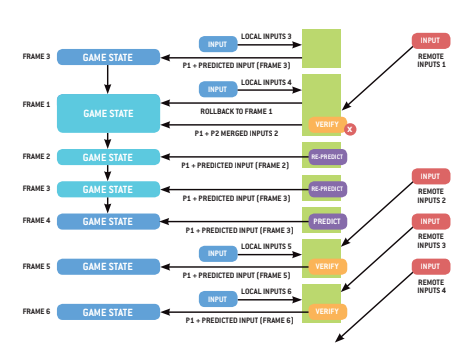
\includegraphics{RollbackNetcodeRepresentation}
\caption{Rollback netcode \cite{GGPODocumentation}}
\label{fig:RollbackNetcodeRepresentation}
\end{figure}
\newpage
\subsection{Difficulties in industry}
In today's fighting game market, many games have rollback \cite{GamesWithRollback}.However there are still notable exceptions such as:
\begin{itemize}
\item Super Smash Bros. Ultimate\cite{SSBU}
\item Granblue Fantasy Versus\cite{GBFV}
\item Under Night In-Birth\cite{UNI}
\item Samurai Shodown\cite{SamSho}
\item Soulcalibur VI\cite{SVI}
\item Dead or Alive 6\cite{DOA6}
\item EA Sports UFC 4\cite{UFC4}
\item Dragon Ball FighterZ\cite{DBFZ}
\end{itemize}

Other fighting games have had difficulty in implementing rollback, such as Street fighter V and Mortal Kombat X.
These difficulties with implementing and developing rollback are the basis of the motivation of this paper.

\subsection{Aim}
To investigate rollback netcode, it's usage in industry and any short comings of existing public rollback netcode infrastructure
\subsection{Objectives}
\begin{itemize}
\item Understand rollback netcode and the effects on the games it's implemented in.
\item Create a visualization for the differences between rollback and delay based netcode.
\item Research the difficulties of implementing rollback in existing games.
\item Explore optimizations for the existing public rollback structure.
\item Investigate further uses of rollback netcode, in the wider video game industry.
\end{itemize}
\newpage
\section{Background}
\subsection{Peer to Peer Netcode}
Peer to peer networks over the internet communicate data in packets which can run into the following issues.
\begin{itemize}
\item{Packets take time to reach their destination (Network Latency).}
\item{Packets can get lost on their way (Packet Loss).}
\item{Packets can get there, but have their data corrupted (Corruption).}
\item{Computers can run at different speeds.}
\item{Computers can occasionally get hung up on doing things and skip a frame or two.}
\end{itemize}

In solving these issues, not only does the quality of the user experience for on-line play, but it also allows for more effective matchmaking soultions, by increasing maximum tolerable connection quality.

\subsection{Delay-based netcode}
\subsubsection{Concept}
Delay based netcode works by keeping both players games in lockstep, meaning that each player's simulation of the game are waits for the input of the remote player, before simulating the frame\cite{DelayBasedNetcode}. This system works well when latency is not a major factor, for example, in a turn based game, where the inputs are spread apart by seconds, a pause of half a second may go unnoticed.
Input latency frames are added to compensate for the Network Latency, and allow the local inputs to be sent before the frame they would be read on as shown in figure \ref{fig:InputLatencyEffect}.

\begin{figure}[h]
\centering
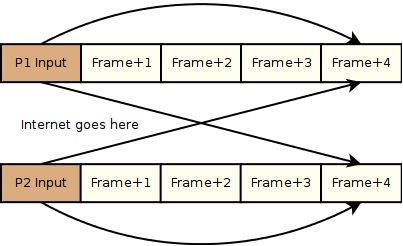
\includegraphics{InputDelay}
\caption{4 Frame Input Delay Example \cite{FightingGameNetworking}}
\label{fig:InputLatencyEffect}
\end{figure}

The Input delay to be used can be calculated as follows:
\[InputLatencyFrames = Ceiling( \frac{RoundTripLatency}{2 * FrameDuration} ) + Constant\]

Where the constant represents additional frames of delay to compensate for variance in Network Latency.

\subsubsection{Improvements}
However this model does not take into account potential for packet loss/ corrupted packets, which may lead the actual states to progress as shown in figure \ref{fig:PacketLossEffect}

\begin{figure}[h]
\centering
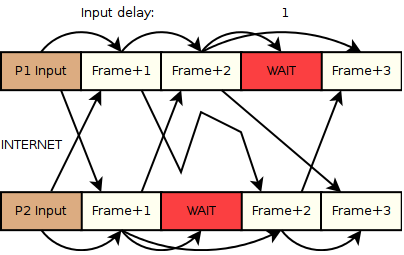
\includegraphics{PacketLossEffect}
\caption{Packet Loss's Affect on Game State progression \cite{FightingGameNetworking}}
\label{fig:PacketLossEffect}
\end{figure}

One unexpected side effect of packet loss with single input packets is knock on delays, where by a delay in one game, makes the frame process later, so the inputs for that frame are postponed, delaying the origins game.

To combat packet loss and data corruption multiple inputs can be sent with one packet, extra frames of input delay can be added, and inputs can be sent multiple times, as shown in \ref{fig:PacketLossSoultions}

\begin{figure}[h]
\centering
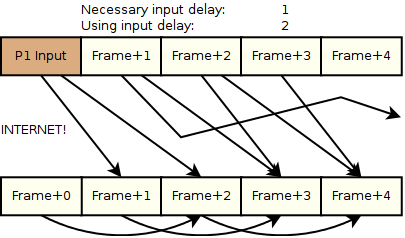
\includegraphics{PacketLossSoultions}
\caption{Potential Solutions to Packet Loss in Delay Based Netcode \cite{FightingGameNetworking}}
\label{fig:PacketLossSoultions}
\end{figure}

Another improvement to made to delay based netcode is to account for Network Latency variance with a dynamic number of delay frames. way to account for Network Latency variance is to have a dynamic number of Delay Frames, varying with average Latency\cite{DelayVsRollback}. This can hide stutters, and remedy degrading network conditions causing consistent pauses. However, consistency for fighting games is the one of the highest determiners on network quality\cite{Core-ARollback}.

\subsubsection{Evaluation}
When there is minimal Network Latency variance, delay based netcode functions similarly to a non networked experience, with increased Input Latency. This is the ideal case for delay based networking. However, when the Network Latency variance is high, the game can freeze at seemingly random moments, removing agency from the player in the middle of a game. This breaks user imersion and significantly decreases the quality of the experience\cite{DelayVsRollback}.

Ultimately Delay based netcode functions as network soultion for high quality connections, but struggles when operating as connection quality degrades. \cite{KIInterview}.
\subsection{Rollback netcode}
\subsubsection{Concept}
Rollback netcode takes the existing framework of delay based netcode and builds on top of it. Instead of waiting for the remote user's input to simulate a frame, the game predicts it.  is These predictive frames By not requiring the input of the remote user to simulate a frame, it can tolerate late and lost packets better than delay based \cite{GGPODocumentation}. When a packet is lost or late, the rollback frames act as a buffer preventing the from game freezing.

\subsubsection{Extra functionality required}
Implementing rollback is not as simple as just changing your existing networking solution, these things need to be added
\begin{itemize}
\item separate gameplay from rendering
\item serializable game state
\item loadable game state
\item game state simulation for multiple frames in the duration (time) of a single frame
\end{itemize}
\subsubsection{Issues In theory}
Because rollback doesn't require the remote user's input to simulate the frame, it comes with it's own associated issues.
\begin{itemize}
\item Particle Simulation.
Because particles are often expensive computationally to process, so preventing deletion of the particles until the roll-back buffer expiries, and only generating them until their existence is confirmed from a remote input
\item Sound Effects
Typically sound effects are loaded as files and sent to audio drivers, with no ability to pause the effect or play from a specific time stamp. To allow for rollback without jarring audio effects they will have to be handled differently.
\item Desync Detection
Naturally rollbacks occur because the remote input state (and thus game state) disagrees with the local game state. Desyncs in rollback netcode happen when confirmed ( non-rollback) frames differ.
\item Optimization
Because rollbac can require the simulation of multiple game state frames in the space of a normal frame duration, the game will likely have to have the capability to process game state updates faster than delay based solutions.
\end{itemize}
\subsection{Evaluation}
Ultimately Rollback on paper seems like a superior solution for fighting games as shown in the figure \ref{fig:NetcodeCompare}.  
table from {https://youtu.be/7jb0FOcImdg?t=623}

\begin{figure}[h]
\centering
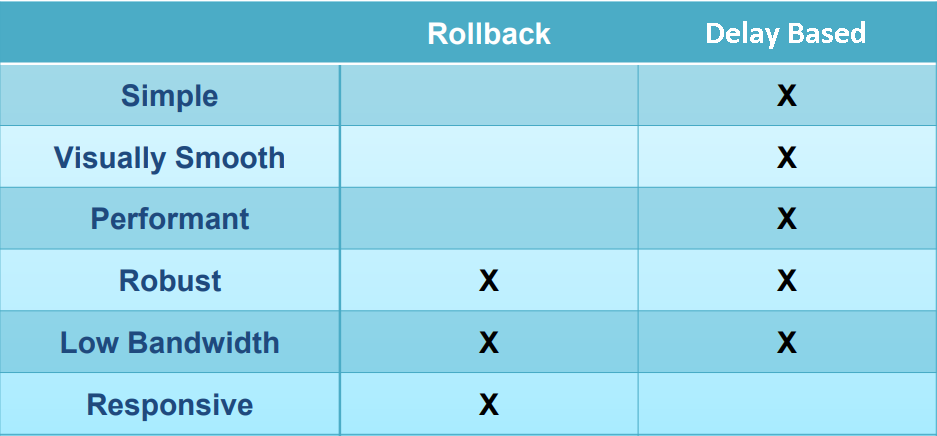
\includegraphics[width=\textwidth]{NetcodeCompare}
\caption{Table comparing differences between Rollback and Delay Based Netcode\cite{8Frames}}
\label{fig:NetcodeCompare}
\end{figure}

Made even easier to implement given an open source solution under the MIT licence \cite{GGPODocumentation}. 
\section{Industry Issues}
However the fighting game industry has had significant difficulty in adopting rollback netcode into their games \ref{sec: introduction}. In this section, Street Fighter V and Mortal Kombat X are analysed, to understand the issues they had with implementation of rollback.
\subsection{Street Fighter V}
Street Fighter V(SFV)'s rollback netcode was released to the public to widespread disappointment \cite{Netcode 1} \cite{Netcode 2} \cite {Netcode 3} \cite {Netcode 4} \cite{Core-ARollback}.  The following issues were found with SFV's rollback:
\begin{itemize}
\item One Sided rollback. \cite{SFV 1}  \cite{SFV 2} \cite {SFV 3}
One sided rollback is when two game states drift out of sync, through either a series of lost packets, or one machine failing to keep up to 60FPS. So for one client, they will receive extremely frequent rollbacks. Whilst the other client will not receive any rollbacks as shown in figure \ref{fig:OneSided}
\begin{figure}[h]
A network with 1 frame Input Latency and 1 Rollback frame.
\resizebox{\textwidth}{!}{
\begin{tabular}{c|c|c|c|c}
\multicolumn{2}{c|}{User 0} & & \multicolumn{2}{c}{User 1} \\
\hline
Local Frame & Local Network Events & & Local Network Events & Local Frame\\
\hline
0 & Send 0's input for frame 0 && Send 1's input for frame 1 & 0 \\
\hline
1 & Send 0's input for frame 1 && Send 1's input for frame 1(Lost) & 1 \\
1 & Receive 1's input for frame 0 && Receive 0's input for frame 0 & 1 \\
\hline
2 & Send 0's input for frame 2 && Send 1's input for frame 2(Lost) & 2 \\
2 & Guesses 1's input for frame 1 && Receive 0's input for frame 1 & 2 \\
\hline
3 & Send 0's input for frame 3 && Send 1's input for frame 3(Lost) & 3 \\
3 & Halt for 1's input from frame 1 && Receive 0's input for frame 2 & 3 \\
\hline
3 & Send 0's input for frame 3 && Send 1's input for frame 4 & 4 \\
3 & Receive 1's input for frame 1,2 and 3 (Rollback) && Receive 0's input for frame 3 & 4 \\
\hline
4 & Sends 0's input for frame 4 && Sends 1's input for frame 4 & 5 \\
4 & Receive 1's input for frame 4 && Guesses 0's input for frame 3 & 5 \\
\end{tabular}
}
\caption{A demonstration of how onesided rollback occurs}
\label{fig:OneSided}
\end{figure}
\item Dynamic Delay frames. \cite{SFV 1}
Dynamic delay frames can make a game feel slow despite having no freezing, because it's hard to feel how long after a button is pressed, that its effect happens on screen.
\item Large effects faster than rollback buffer. \cite{SFV 1}
If there are large effects that get rollback over or rollback into the effect can be very jarring for the player.
\end{itemize}


From These issues we can learn the following lessons.
\begin{itemize}
\item How to fix one sided rollback.
\item Static Delay frames.
\item Make sure events are confirmed before large effects
\end{itemize}
\subsection{Mortal Kombat X}
Mortal Kombat X (MKX) was released in 2015 with delay based netcode. Rollback netcode was added in a patch to the game in 2018. However there are les
Issues:
Manpower
Performance

Lessons Learnt:
Identify QOS cut off (max ping)
Performance tricks  
Added after lauch, huge performance issues solved with:
Multithreading, improved object handling (deferred deletion), evaulation of fixed cost, profiling tools !, optimizing game play loop as it in the worst case is going to be replayed multiple times.
Turn off predictable(?) things each frame (by predictable I mean, f(sum(inputs)) = sum(f(inputs)).
Need a seperate resimulated gameplay loop (desync detection).
Only need to save confirmed frame (good for worst, bad for average) (save simulation mid point calculate performance based on rollback frame and particles generated this frame)
precompute!
Really fuzzy matching on non gameplay effecting effects i.e. audio, particles with no hitboxes
Game rollback max really infrequently. Humans input speed max = find sc2 max apm
Possible to slow fps of game if struggling to get performance instead of pausing
Design systems to update with variable time steps
defer processing until guaranteed response i.e. camera cuts, particle spawning
7/8 man years to implement (4/5 optimization, 1/2 serialization,


\section{Rollback Visualization tool}
To demonstrate the effectiveness of Rollback vs Delay based netcode, a simulation of the two different styles of netcode was made.
\subsection{Design}
The high level design of this visualization tool was to have two side by side game clients, communicating to each other through simulated latency and netcode. Because the visualization tool was just supposed to be a demonstration, no overly complex mechanics would be implemented. It would just be two avatars that could move and jump.

Unity was chosen as the engine to develop the simulation, as designing from an existing game engine, would make development faster, and the developer had experience in using unity before.

The user would have the options to change the effect of network latency on the simulation(s) in real time, and the properties of the netcode, such as Input Latency, Rollback frames and packet loss \%. 
The overall design of the visualization tool is shown in figure \ref{fig:DFD}.

\begin{figure}[h]
\centering
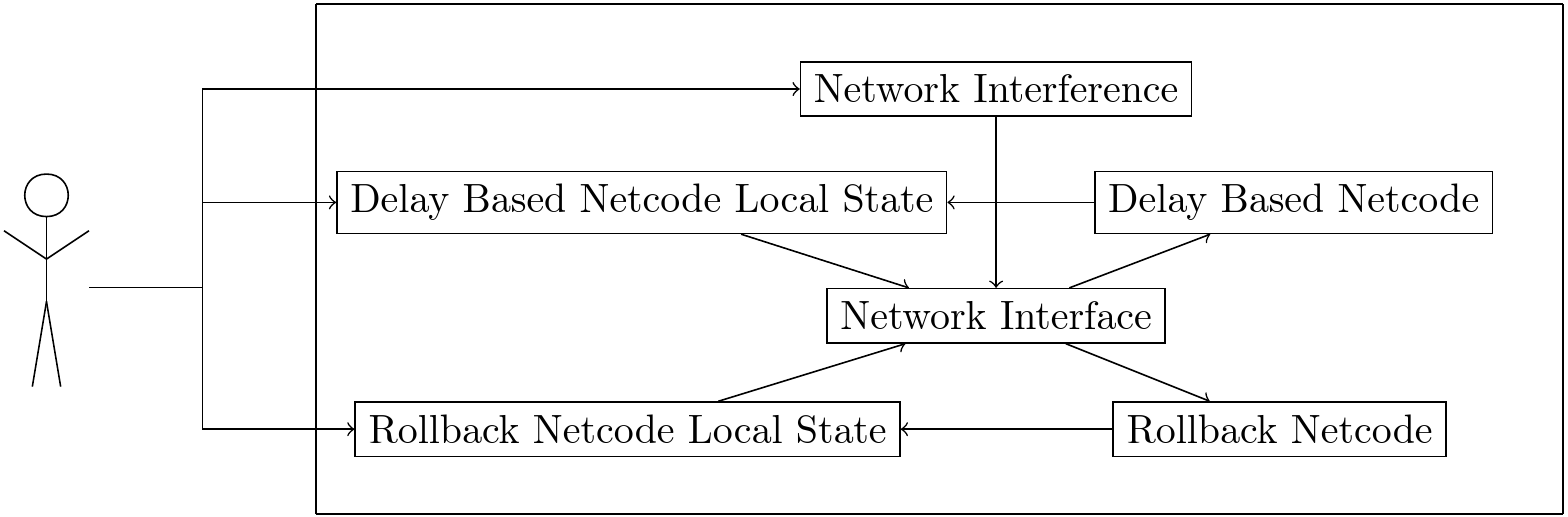
\includegraphics[width=\textwidth]{UIDesign}
\caption{Data Flow Diagram for Rollback Visualization tool}
\label{fig:DFD}
\end{figure}

\subsection{Implementation}

Initially the packet structure was chosen to be a single frame's input, however during development I realized that the packet structure improvements mentioned in \ref{sec: Background} could be applied to combat packet loss.

State serialization was surprising simple, as the only two dynamic elements of my game were the two players. Meaning that the only properties I had to save would be their location and velocity. If the game had more functionality, such as a health system, or audio effects, which are present in most modern games, extra systems would have had to be implemented on top to support dynamic saving and loading of state.

Experiment With packet loss solutions


How seperate rendering from game state in unity? = Don't allow render texture to update


If a players inputs cannot change the state, then the simulation can continue without them. This can be used to slightly reduce the average amount of rollbacks and freezes in both netcode implementations. To implement this idea, a frames till actionable variable was added to the packet data, and the delay based netcode would not freeze for the remote user's inputs / rollback would not re-simulate frames if the guessed inputs were different whilst the frames till actionable value was larger than 0. This could also have further adaption in rollback netcode, where only a certain number of the remote's inputs could matter, minimizing potential rollbacks.


I noticed desyncs happening, between my adjacent simulations, despite inputs being identical. In order to try to fix this, I made more thorough re-jump detection, reducing parallelization in the code, manually ran physics updates for a set duration in stead of relying upon unity's fixed updates. Ultimately to no prevail. So I had to chose between redesigning unity's physics engine (the presumed source of lack of determinism) for deterministic behaviour or re-designing my visualization tool. I chose redeisgn as I could felt I could demonstrate the difference in delay based and rollback netcode from a users experience, if they were allowed to toggle between the different types of netcode.

reworked design

Networked state
 |                  \
\ /                  \
 V                    Netcode handler (recives input from game states and handles communication between them) - Network interfence customiser, Rollback, delay based, remote input
1 game states              
/             \                        \
1 local player   1 remote player        local input
 remote input subclass of local input

made own fixed size buffer class to prevent excess memory being used
Rollback always saving state, so if swap, can load prior states
Delay based code explained
Rollback code explained
pause game when rollbacks happen

having issues with frames taking longer than 16ms (Turns out unity overhead)
simulate max rollbacks 100\% of time
needed extra for game state from rollback explained

Buffer sizes?

Implement ideas from delay based netcode packet soultions = expanded packet size

\subsection{Evaluation}
Unity no determinism (redo engine?)
Rollback hard even for simple projects
Didn't implement Audio or particle systems
Better ping modelling
This simulation could also allow for testing of various improvements of the netcodes, such as multiple packet sending, increasing frames sent, etc.

\section{Improvements for Rollback}



\subsection{Prediction Quality}
https://www.diva-portal.org/smash/record.jsf?pid=diva2%3A1560069&dswid=-2962  -> neural networks

-Naive is ~90\% accurate {https://www.youtube.com/watch?v=k9JTIn1SVQ4\&t=1888s}
hard to run expensive algorithms alongside large rollbacks (cite MKX talk)

\subsection{Packet Contents Optimization}
Delay based strategies
How many frames to send, request for frame? = delay frames? + constant?

I propose a theory for rollback frames 
\[rollback frames = ceiling{max acceptable ping}{2*frameduration} - delay frames)\]
for dynamic: dynamically changing rollback = minimal effect, (Problem with maxing rollback? = Divergence and hardware doesn't support rolling back that far in 1 frame (16ms))
however try to keep delay static \cite{sec:Industry Issues}

\subsection{Input Locking}
No need for rollbacks when input doesn't matter, i.e. hit stun, hit pause, cutscene, jumping, in a move past a cancel window \cite{sec:Industry Issues}

\subsection{Conclusion}
These require further testing

\section{Wider use case of rollback netcode}
Rollback ideas that only apply to fighting games? (Visual teleportation?, Expensive to implement?, ) 
 RTS (Including sports games)
FPS - https://ieeexplore.ieee.org/abstract/document/7991545
Prediction quality:
- Connection ‘quality’. This doesn’t mean bandwidth, but rather how much a connection’s response time fluctuates. This has improved in modern times, making rollback a much more viable option than it once was.
- The type of game. Because rollback needs you to be able to revert the state of the game in some cases, trying to implement it in a game with hundreds of different units all acting at once is extremely challenging (not to mention very offputting for the player). As a result, it’s more suited to fighting games and other games with fewer player-controlled assets flying around at any given time.


\section{Conclusions and further work}

Overall rollback hard to implement, but not impossible, newer games not releasing without it. Lessons learnt. Probably not applicable for wider use case. 

furture work: 
Non-game applications? Expand upon demo
\begin{thebibliography}{25}

\bibitem{GGPODocumentation} {\texttt https://drive.google.com/file/d/1nRa3cRBQmKj0-SEyrT\_1VNOkPOJWNhVI/view} or 
{\texttt https://web.archive.org/web/20220101162600/https://drive.google.com/file/d/1nRa3cRBQmKj0-SEyrT\_1VNOkPOJWNhVI/view} 
Tony C., GGPO Game Developer Magazine's article. 2012. (Visited 25/05/2022)

\bibitem{FGCMajors} {\texttt https://liquipedia.net/fighters/Tier\_1\_Tournaments} or 
{\texttt https://web.archive.org/web/20210121113554/https://liquipedia.net/fighters/Tier\_1\_Tournaments} 
Liquidpedia list of major fighting game tournaments. (Visited 25/05/2022)

\bibitem{FirstUSTournament} {\texttt https://www.usgamer.net/articles/the-oral-history-of-evo} or 
{\texttt https://web.archive.org/web/20220321000753/https://www.usgamer.net/articles/the-oral-history-of-evo} 
John L., The Oral History of EVO: The Story of the World's Largest Fighting Game Tournament (Visited 25/05/2022)

\bibitem{FGCAsEsport} {\texttt https://esportsinsider.com/2021/10/can-fighting-games-become-a-mainstream-esport/} or 
{\texttt https://web.archive.org/web/20220516060805/https://esportsinsider.com/2021/10/can-fighting-games-become-a-mainstream-esport/} 
Elizbar R., Can fighting games become a mainstream esport without abandoning grassroots?. (Visited 26/02/2022) 

\bibitem{SmashTournamentsInThePandemic} {\texttt https://www.ssbwiki.com/COVID-19\_pandemic\_and\_its\_impact\_on\_competitive\_Smash} or {\texttt https://web.archive.org/web/20220516020551/https://www.ssbwiki.com/COVID-19\_pandemic\_and\_its\_impact\_on\_competitive\_Smash} List of smash tournaments affected by the pandemic. (Visited 26/02/2022) 

\bibitem{GuiltyGearStriveInThePandemic} {\texttt https://techraptor.net/gaming/opinions/guilty-gear-strive-changed-fighting-games-rollback-netcode} or {\texttt https://web.archive.org/web/20210713144527/https://techraptor.net/gaming/opinions/guilty-gear-strive-changed-fighting-games-rollback-netcode} Davi B. Guilty Gear Strive Might Have Changed Fighting Games Forever. (Visited 26/02/2022)

\bibitem{DelayVsRollback} {\texttt https://arstechnica.com/gaming/2019/10/explaining-how-fighting-games-use-delay-based-and-rollback-netcode/} or {\texttt https://web.archive.org/web/20220425211823/https://arstechnica.com/gaming/2019/10/explaining-how-fighting-games-use-delay-based-and-rollback-netcode/} Ricky P. Explaining how fighting games use delay-based and rollback netcode. (Visted 26/05/2022)

\bibitem{BadNetcode} {\texttt https://www.polygon.com/2020/3/25/21192522/netcode-samurai-showdown-fighting-games-rollback-delay} or {\texttt https://web.archive.org/web/20220401231646/https://www.polygon.com/2020/3/25/21192522/netcode-samurai-showdown-fighting-games-rollback-delay} David C. Bad netcode is killing many of your favorite fighting
games. (Visted 26/05/2022)

\bibitem{RollbackDevelopment} {\texttt https://gamasutra.com/view/news/34050/Interview\_How\_A\_Fighting\_Game\_Fan\_Solved\_Internet\_Latency

\_Issues.php} or {\texttt https://web.archive.org/web/20220325062609/https://gamasutra.com/view/news/34050/
Interview\_How\_A\_Fighting\_Game\_Fan\_Solved\_Internet\_Latency\_Issues.php} Kyle O. Interview: How A Fighting Game Fan Solved Internet Latency Issues. (Visted 26/05/2022)

\bibitem{FightingGameDefine} {\texttt https://archive.org/details/nextgen-issue-015/page/n33/mode/2up} "The Next Generation 1996 Lexicon A to Z: Fighting Game". (Visited 26/05/2022)

\bibitem{DelayBasedNetcode} {\texttt https://www.gamasutra.com/view/feature/3094/1500\_archers\_on\_a\_288\_network\_.php} or {https://web.archive.org/web/20220506231117/https://www.gamasutra.com/view/feature/3094/
1500\_archers\_on\_a\_288\_network\_.php} Mark T. 1500 Archers on a 28.8: Network Programming in Age of Empires and Beyond. (Visted 26/05/2022)

\bibitem{FightingGameNetworking} {\texttt https://web.archive.org/web/20210228051849/https://mauve.mizuumi.net/2012/07/05/understanding-fighting-game-networking.html} Mauve M. Understanding Fighting Game Networking. (Visted 26/05/2022)

\bibitem{GamesWithRollback} {\texttt https://attackofthefanboy.com/guides/rollback-netcode-games-list/} or {\texttt https://web.archive.org/web/20211122034207/https://attackofthefanboy.com/guides/rollback-netcode-games-list/} Andron S. Rollback Netcode Games List (March 2022). (Visted 26/05/2022)

\bibitem{SSBU} {\texttt https://en.wikipedia.org/wiki/Super\_Smash\_Bros.\_Ultimate} or {\texttt https://web.archive.org/web/20220519200835/https://en.wikipedia.org/wiki/Super\_Smash\_Bros.\_Ultimate} Super Smash Bros. Ultimate. (Visited 26/05/2022)

\bibitem{GBFV} {\texttt https://en.wikipedia.org/wiki/Granblue\_Fantasy\_Versus} or {\texttt https://web.archive.org/web/20220512125807/https://en.wikipedia.org/wiki/Granblue\_Fantasy\_Versus} Grandblue Fantasy Versus (Visited 26/05/2022)

\bibitem{UNI} {\texttt https://en.wikipedia.org/wiki/Under\_Night\_In-Birth} or {\texttt https://web.archive.org/web/20220516020108/https://en.wikipedia.org/wiki/Under\_Night\_In-Birth} Under Night In-birth (Visited 26/05/2022)

\bibitem{SamSho} {\texttt https://en.wikipedia.org/wiki/Samurai\_Shodown\_(2019\_video\_game)} or {\texttt https://web.archive.org/web/20220504020927/
https://en.wikipedia.org/wiki/Samurai\_Shodown\_(2019\_video\_game)} Samurai Shodown (Visited 26/05/2022)

\bibitem{SVI} {\texttt https://en.wikipedia.org/wiki/Soulcalibur\_VI} or {\texttt https://web.archive.org/web/20220421074040/https://en.wikipedia.org/wiki/Soulcalibur\_VI} Soulcalibur VI (Visited 26/05/2022)

\bibitem{DOA6} {\texttt https://en.wikipedia.org/wiki/Dead\_or\_Alive\_6} or {\texttt https://web.archive.org/web/20220130144906/https://en.wikipedia.org/wiki/Dead\_or\_Alive\_6} Dead or Alive 6 (Visited 26/05/2022)

\bibitem{UFC4} {\texttt https://en.wikipedia.org/wiki/EA\_Sports\_UFC\_4} or {\texttt https://web.archive.org/web/20211019192531/https://en.wikipedia.org/wiki/EA\_Sports\_UFC\_4} EA Sports UFC 4 (Visited 26/05/2022)

\bibitem{DBFZ} {\texttt https://en.wikipedia.org/wiki/Dragon\_Ball\_FighterZ} or {\texttt https://web.archive.org/web/20220424200258/https://en.wikipedia.org/wiki/Dragon\_Ball\_FighterZ} Dragon Ball FighterZ (Visited 26/05/2022)

\bibitem{Core-ARollback} {\texttt https://www.youtube.com/watch?v=0NLe4IpdS1w} or {\texttt https://web.archive.org/web/20220529231214/https://www.youtube.com/watch?v=0NLe4IpdS1w} Core A Gaming. Analysis: Why Rollback Netcode Is Better. (Visted 31/05/2022)

\bibitem{KIInterview} {\texttt https://www.youtube.com/watch?v=1RI5scXYhK0} or {\texttt https://web.archive.org/web/20220330062542/https://www.youtube.com/watch?v=1RI5scXYhK0} Hold Back To Block. Talking Netcode With Adam "Keits" Heart (Visited 31/05/2022)

\bibitem{InputLatencyDatabase} {\texttt https://displaylag.com/video-game-input-lag-database/} or {\texttt https://web.archive.org/web/20220519183335/https://displaylag.com/video-game-input-lag-database/} Display Lag. Video Game Input Lag Database. (Visted 02/06/2022)

\bibitem{8Frames} {\texttt https://www.gdcvault.com/play/1025021/8-Frames-in-16ms-Rollback} or {\texttt https://web.archive.org/web/20210819020226/https://www.gdcvault.com/play/1025021/8-Frames-in-16ms-Rollback} Michael S. 8 Frames in 16ms: Rollback Networking in 'Mortal Kombat' and 'Injustice 2'. (Visted 08/06/2022)

\bibitem{Netcode 1} {\texttt https://www.eventhubs.com/news/2022/jan/09/3-problems-sf5-netcode/} Jon G. 3 major problems with Street Fighter 5's netcode I want fixed. (Visted 08/06/2022)

\bibitem{Netcode 2} {\texttt https://litetheironman.medium.com/street-fighter-v-and-rollback-netcode-101-8921a1e8a1c6} Nathan D. Street Fighter V and Rollback Netcode 101. (Visted 08/06/2022)

\bibitem{Netcode 3} {\texttt https://www.youtube.com/watch?v=iGgG6eWk1Xo} Brian F. Why SFV Netcode Sucks. (Visted 08/06/2022)

\bibitem{Netcode 4} {\texttt https://egmnow.com/street-fighter-v-has-finally-fixed-its-netcode-but-a-modder-did-it-first/} Dave M. Street Fighter V Has Finally Fixed Its Netcode—But a Modder Did It First. (Visted 08/06/2022)

\bibitem{SFV 1} {\texttt https://www.youtube.com/watch?v=OtSveL7X6xg} DigitalHalftones.  Altimor's SFV Netcode Fix Mod Visually Explained. (Visted 08/06/2022)

\bibitem{SFV 2} {\texttt https://www.youtube.com/watch?v=9ENocn-x0Ws} fluffysheap. SFV Netcode Fix. (Visted 08/06/2022)

\bibitem{SFV 3} {\texttt https://github.com/https://github.com/fluffysheap/SFVNetcodeFix/SFVNetcodeFix} fluffysheap. SFV Netcode Fix. (Visted 08/06/2022)

\end{thebibliography}
\end{document}
